\documentclass{article}
\usepackage[utf8]{inputenc}

\usepackage{sectsty}
\usepackage{fancyhdr}
\usepackage[top=1.25cm, bottom=2cm, left=2cm, right=2cm]{geometry}
\usepackage{tabularx,tabulary}
\usepackage{graphicx}
\date{Lundi 11 Mars 2019}
\author{FRANCESCHETTI Maël\\KADOCH Daoud\\MANSON Fabien\\CASTANET Nicolas}
\title{\LARGE{Projet 3i013\\}Cahier des Charges}

\usepackage[french]{babel}
%\usepackage[utf8x]{inputenc}
%\usepackage{amsmath}
%\usepackage[colorinlistoftodos]{todonotes}
\begin{document}

\begin{titlepage}

\newcommand{\HRule}{\rule{\linewidth}{0.5mm}} % Defines a new command for the horizontal lines, change thickness here

\center % Center everything on the page
 
%----------------------------------------------------------------------------------------
%	HEADING SECTIONS
%----------------------------------------------------------------------------------------

\textsc{\LARGE Université Pierre-et-Marie-Curie}\\[3cm] % Name of your university/college
\textsc{\Large Licence Informatique 3\up{ème} Année}\\[0.5cm] % Major heading such as course name
\textsc{\large Projet 3i013}\\[2cm] % Minor heading such as course title

%----------------------------------------------------------------------------------------
%	TITLE SECTION
%----------------------------------------------------------------------------------------

\HRule \\[0.4cm]
{ \huge \bfseries Cahier des Charges}\\[0.4cm] % Title of your document
\HRule \\[2cm]
 
%----------------------------------------------------------------------------------------
%	AUTHOR SECTION
%----------------------------------------------------------------------------------------

\begin{minipage}{0.4\textwidth}
	\begin{flushleft} \large
	\emph{Auteurs:}\\[0.2cm]
	Nicolas \textsc{CASTANET}\\ % Your name
	Maël \textsc{FRANCESCHETTI}\\ % Your name
	Daoud \textsc{KADOCH}\\ % Your name
	Fabien \textsc{MANSON} % Your name
	\end{flushleft}
\end{minipage}
~
\begin{minipage}{0.4\textwidth}
	\begin{flushright} \large
	\emph{Enseignant:} \\[0.2cm]
	Fabrice \textsc{KORDON}
	\end{flushright}
\end{minipage}\\[4cm]

%----------------------------------------------------------------------------------------
%	DATE SECTION
%----------------------------------------------------------------------------------------

{\large Lundi 11 Mars 2019}\\[3cm] % Date, change the \today to a set date if you want to be precise

%----------------------------------------------------------------------------------------
%	LOGO SECTION
%----------------------------------------------------------------------------------------


\includegraphics[scale=0.15]{logo_sorbonne.png} % Include a department/university logo - this will require the graphicx package
 
%----------------------------------------------------------------------------------------

\vfill % Fill the rest of the page with whitespace

\end{titlepage}

% -----------------------------------------------------
\newpage
\renewcommand{\contentsname}{\center{Table des Matières}\vspace*{5cm}}

\tableofcontents



\newpage
\section{Présentation du Projet}
	\subsection{Contexte et définition du problème}
		Un client nous contacte dans le but de réaliser une application lui permettant d'effectuer un vol autonome avec un drone Bebop 2 tout en visualisant sur un iPod Touc le retour vidéo de la caméra embarquée sur le drone. L'iPod sera placé dans un masque de vue à la première personne. \\	
		%Le client souhaite faire effectuer des vols autonomes à un drone Bebop 2, avec un retour vidéo en temps réel sur un iPod Touch. Ce dernier pourra être placé dans un masque de vue à la première personne.\\
		La solution devra permettre à l'utilisateur de saisir un plan de vol sur une carte interactive et de le faire exécuter par le drone tout en ayant un retour vidéo sur l'iPod.\\
		\medbreak
        \begin{flushleft}
	    \textbf{Cas d'utilisation :} \\
	    \end{flushleft}
	    \begin{flushleft}
	    1) Un utilisateur souhaite effectuer une ronde avec un drone pour surveiller sa propriété (qui possède un très grand jardin) au prix d'un moindre effort.\\
	    Voici un exemple des étapes qu'il va suivre chronologiquement :\\
		[1cm]	     
	    \end{flushleft}
	    \begin{center}
	    \renewcommand{\arraystretch}{2}
        \begin{tabularx}{15cm}{|c|X|}
            \hline
            1 & L'utilisateur lance l'application et arrive sur la page d'accueil.\\
            \hline
            2 & L'utilisateur lance la fonctionnalité de saisie du plan de vol sur une machine connectée au réseau local.\\
            \hline
            3 & L'utilisateur saisit le plan de vol sur la carte en spécifiant les points de passage du drone ainsi que les altitudes que le drone doit adopter au cours du vol. \\
            \hline
            4 & L'utilisateur valide la saisie de son plan de vol, ce dernier est enregistré. \\
            \hline
            5 & L'utilisateur allume le drone et y connecte sa machine en wifi. \\
            \hline
            6 & L'utilisateur lance la fonctionnalité d'exécution du plan de vol. \\
            \hline
            7 &  L'utilisateur démarre l'iPod touch, le connecte au réseau local et lance l'application de réception vidéo. La réception vidéo en temps réel sur l'iPod commence.\\
            \hline
            8 & L'utilisateur sélectionne parmi les plans de vols présents sur le drone celui qu'il vient de réaliser. \\
            \hline
            9 & L'utilisateur place l'iPod dans le masque FPV, le met sur sa tête, puis lance l'exécution du plan de vol. Le drone décolle. \\
            \hline
            10 & Le drone effectue le plan de vol choisi, l'utilisateur voit en temps réel ce que le drone filme. \\
            \hline
            11 & L'utilisateur souhaite stopper l'exécution de plan de vol : par exemple, il a repéré quelque chose d'anormal sur la zone de vol et souhaite s'y rendre au plus vite. Il active alors la procédure d'arrêt d'urgence sur sa machine et retire le masque FPV. Le drone stoppe l'exécution du plan de vol et attérit sur place si les conditions le permettent. \\
            \hline
        \end{tabularx}
        \end{center}
        
        \newpage
        \begin{flushleft}
        2) En hiver, un utilisateur souhaite faire effectuer au drone le tour de son jardin pour contrôler le niveau d'enneigement de celui-ci sans risquer de glisser.\\
        Voici un exemple des étapes qu'il va suivre chronologiquement : \\ [1cm]
        \end{flushleft}
	    \begin{center}
	    \renewcommand{\arraystretch}{2}
        \begin{tabularx}{15cm}{|c|X|}
            \hline
            1 & L'utilisateur lance l'application et arrive sur la page d'accueil.\\
            \hline
            2 & L'utilisateur lance la fonctionnalité de saisie du plan de vol sur une machine connectée au réseau local.\\
            \hline
            3 & L'utilisateur saisit le plan de vol sur la carte en spécifiant les points de passage du drone tout autour de son jardin et spécifie une altitude de quelques mètres. Le tracé est fait de manière à faire revenir le drone à son point de départ après avoir fait le tour du jardin. \\
            \hline
            4 & L'utilisateur valide la saisie de son plan de vol, ce dernier est enregistré. \\
            \hline
            5 & L'utilisateur allume le drone et y connecte sa machine en wifi. \\
            \hline
            6 & L'utilisateur lance la fonctionnalité d'exécution du plan de vol. \\
            \hline
            7 &  L'utilisateur démarre l'iPod touch, le connecte au réseau local et lance l'application de réception vidéo. La réception vidéo en temps réel sur l'iPod commence.\\
            \hline
            8 & L'utilisateur sélectionne parmi les plans de vols présents sur le drone celui qu'il vient de réaliser. \\
            \hline
            9 & L'utilisateur place l'iPod dans le masque FPV, le met sur sa tête, puis lance l'exécution du plan de vol. Le drone décolle. \\
            \hline
            10 & Le drone effectue le plan de vol choisi, l'utilisateur voit en temps réel ce que le drone filme et peut constater l'état d'enneigement de son jardin. \\
            \hline
            11 & L'utilisateur attend la fin de l'exécution du plan de vol pour retirer le masque et aller récupérer le drone une fois qu'il aura atterri à son point de départ, comme prévu.\\
            \hline 
        \end{tabularx}
        \end{center}
        \vspace*{1cm}
	\subsection{Objectifs}
		%\vspace*{0.3cm}
		\begin{enumerate}
        	\item Permettre à l'utilisateur de saisir un plan de vol étape par étape sur une carte interactive et de spécifier les altitudes du drone à chaque point de passage.
        	\item Permettre à l'utilisateur de sauvegarder son plan de vol pour le réutiliser plus tard.
			\item Permettre à l'utilisateur de lancer l'exécution du plan de vol réalisé au préalable.
		 	\item Rediriger le flux vidéo du drone vers l'iPod touch. 
		 	\item Minimiser les latences vidéo (de l'ordre de la seconde).
		 	\item Permettre d'arrêter le vol en cours en cas d'urgence.
		\end{enumerate}
		
\section{Besoins fonctionnels}
	    \begin{center}
	    \vspace*{0.7cm}
        \begin{tabularx}{15cm}{|c|p{4cm}|X|}
            \hline
            1 & Saisie du plan de vol & L'utilisateur doit pouvoir saisir un plan de vol sur une carte à travers une interface intuitive. L'utilisateur doit pouvoir spécifier l'altitude du drone à chaque waypoint (point de passage).\\
            \hline
            2 & Traduction du plan de vol au format Mavlink & Le plan de vol saisi graphiquement par l'utilisateur doit être converti au format Mavlink pour être ensuite envoyé au drone.\\
            \hline
            3 & Envoi du plan de vol au drone & La solution doit prendre en charge la récupération du plan de vol réalisé au préalable et son envoi au drone. \\
            \hline
            4 & Choix du plan de vol  & L'utilisateur doit pouvoir choisir le plan de vol enregistré sur le drone qu'il souhaite exécuter. \\
            \hline
            5 & Exécution du plan de vol  & Une fois le plan de vol choisi, l'utilisateur doit pouvoir en lancer l'exécution. \\
            \hline
            6 & Retour vidéo  & Tout au long du vol du drone, le retour vidéo de ce dernier doit être envoyé sur un iPod touch en temps réel et avec une latence minimale. \\
            \hline
            7 & Arrêt d'urgence  & À tout moment un deuxième utilisateur doit pouvoir enclencher un arrêt d'urgence depuis le PC. \\
            \hline
            8 & Démarrage de la ronde à l'aide de gestes & L'utilisateur pourra éventuellement engager le démarrage du vol en effectuant un certain mouvement de la tête. 	\\
			\hline
			9 & Arrêt d'urgence à l'aide de gestes & L'utilisateur pourra éventuellement engager un arrêt d'urgence en effectuant un certain mouvement de la tête. 	\\
			\hline
        \end{tabularx}
        \end{center}
	
		
\section{Périmètre}
	\subsection{À qui s'adresse le produit ?}
		Ce projet est destiné à un public désirant effectuer une ronde d'une durée de 20 à 25 minutes maximum avec son drone.\\
		La portée maximale du drone est de 200 mètres pour une altitude de 100 mètres tout au plus.
	
	\subsection{Les Limites}
		Le drone ne sera pas capable d'éviter les obstacles durant sa ronde, c'est à l'utilisateur d'établir un trajet cohérent avec son environnement.\\
		De plus, dans le cas où le trajet proposé est trop long par rapport à l'autonomie du drone, un simple message d'avertissement sera affiché pour prévenir l'utilisateur, l'application ne sera pas en mesure d'empêcher cette ronde.
	
	

	
\section{Ressources}
	\subsection{Matériel}
		\begin{flushleft}
	    \textbf{Pour réaliser ce projet nous disposons du matériel suivant :}
	    \end{flushleft}
		\begin{enumerate}
        \item Un drone Bebop 2.
        \item Un iPod Touch de 6ème génération sous iOS 12.
        \item Un accès aux salles machines SAR équipées de machines sous OSX.
        \item un accès aux salles informatiques équipées de machines sous Linux.
        \end{enumerate}
        
	\subsection{L'équipe}

	L'équipe est composée de quatre étudiants en troisième année de licence d'informatique.\\
        Nos connaissances en programmation sous Linux sont bonnes mais le langage Objective-C et l'univers iOS nous sont pour le moment encore inconnus.

\section{Solutions étudiées}
	Au cours de nos recherches nous avons étudié principalement 3 solutions d'architecture envisageables pour le développement de l'application. Ces architectures sont les suivantes, de gauche à droite dans le tableau ci-après (figure 1): 
	  	\begin{enumerate}
        	\item Une architecture utilisant un PC sous linux pour la saisie du plan de vol et qui commande le drone, ainsi qu'un iPod Touch sur lequel on redirige le flux vidéo.
        	\item Une architecture utilisant un iPad pour la saisie du plan de vol, ainsi qu'un iPod Touch qui commande le drone et récupère le flux vidéo.
         	\item Une architecture utilisant un iPod Touch pour la saisie du plan de vol, qui commande le drone tout en récupérant le flux vidéo.\\ \\
        \end{enumerate}
	\subsection{Comparatif des solutions}
	
		%________________		
		\begin{figure}[h]
		\begin{center}
		%\vspace*{0.7cm}
		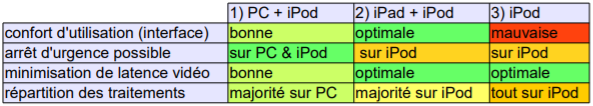
\includegraphics{comparatif_v3.PNG}\\
		\caption{tableau comparatif des solutions}
		\end{center}
		\end{figure}
		%________________
		

		%description précise du tableau        

		\indent Concernant le confort d'utilisation l'avantage est à la seconde solution car l'iPad possède un grand écran ainsi qu'une saisie tactile. La première solution est moins confortable principalement à cause de l'absence de saisie tactile sur le PC. La dernière solution n'est pas très pratique de fait de la petite taille de l'écran de l'iPod.\\
		
        \indent Concernant l'arrêt d'urgence c'est la première solution qui a l'avantage car elle permet d'implémenter cette fonction sur le PC ou sur l'iPod (via un mouvement de tête quand l'utilisateur porte le masque ou la pression d'une touche du clavier). L'arrêt d'urgence sur la troisième solution nous force à implémenter la fonctionnalité via un geste car l'iPod est, rappelons-le, attaché dans le masque donc difficile d'accès. La seconde solution ne pourra pas utiliser l'ipad pour lancer un arrêt d'urgence car l'iPod sera le seul appareil connecté au drone.\\
        
        \indent Les solutions 2 et 3 proposent une latence vidéo réduite car il n'y a pas à rediriger le flux vidéo. Ce dernier est directement reçu et lu par l'iPod. La première solution, en raison de la redirection du flux vidéo depuis le PC vers l'iPod, induit une latence légèrement plus importante (la différence reste assez imperceptible à l'utilisateur).\\
        
        \indent Et finalement en ce qui concerne les traitements réalisés par l'application, dans la première solution la majorité des calculs (saisie du plan de vol, envoie du plan de vol et traitement du flux vidéo reçu) seront fait sur le PC. L'iPod ne fera que recevoir le flux vidéo déjà traité. La seconde solution suit le même principe : la saisie du plan de vol se fait depuis l'iPad mais le traitement du flux vidéo ce fera sur l'iPod. Enfin la dernière solution traitera tout sur l'iPod ce qui peut causer des probleme d'autonomie de batterie pour l'iPod. L'avantage est donc à la première solution.\\ \\
        
        \indent Comme nous pouvons le constater, la solution utilisant le PC et l'iPod Touch est plus avantageuse dans la majorité des cas. C'est donc cette solution qui sera préférée.\\
        
        \indent Voici un schéma de l'architecture générale de la solution que nous avons choisie (figure 2).   
        %________________
 		\begin{figure}[!ht]
 		\begin{center}
 		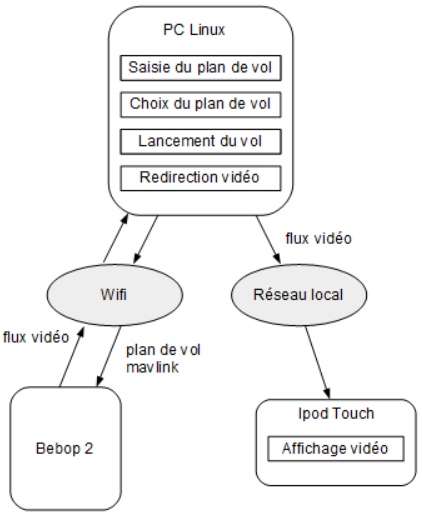
\includegraphics[scale=0.7]{Solution_PC.PNG}
 		\caption{Schéma de l'architecture générale de la solution retenue}
 		\end{center}
		\end{figure}
		%________________
\newpage
\section{Contraintes}

	\begin{flushleft}
	\textbf{Les contraintes techniques de la solution préférée sont :}
	\end{flushleft}
		\begin{enumerate}
        \item Le PC sous Linux doit avoir deux cartes réseau : une pour pouvoir se connecter au drone en wifi, l'autre pour se connecter au réseau local pour rediriger le flux vidéo.
        \item Il faut un réseau local sur lequel sont connectés le PC et l'iPod Touch.
        \item Le réseau local doit avoir un accès internet.
        \end{enumerate}
	
	\subsection{Délais}
		Le cahier des charges doit être envoyé au client pour le lundi 11 mars.\\
		En ce qui concerne le produit, il devra être prêt et livré début mai, et un rapport devra être rendu le jeudi 2 mai avant minuit.\\
		Une soutenance publique devant un jury se tiendra également début mai, nous viendrons y défendre l'ensemble de notre travail.\\
		
	\subsection{Autres contraintes}
	    \begin{flushleft}
	    \textbf{Concernant le plan de vol :} 
	    \end{flushleft}
	    	\begin{enumerate}
            	\item  L'application de saisie du plan de vol doit intégrer une carte interactive permettant de tracer ce dernier.
    		 	\item On devra pouvoir spécifier l'altitude à laquelle le drone doit se trouver aux différents points du parcours.
    		 	\item L'application devra au minimum pouvoir avertir l'utilisateur lorsqu'il tracera un trajet trop long pour le drone, tant pour son autonomie que pour la portée du signal wifi.
		 	\end{enumerate}
		
	    \begin{flushleft}
	    \textbf{Concernant le retour vidéo :}
	    \end{flushleft}
	     	\begin{enumerate}
	     	\item La qualité du retour vidéo est directement liée à la distance avec le serveur central (le PC) ainsi qu'à l'encombrement de l'espace dans lequel le drone vol. Un terrain avec des obstacles comme des bâtiments ou des arbres réduit fortement la porté du signal vidéo.
	     	\item Le retour vidéo du drone doit être envoyé à un iPod Touch en temps réel.
	     	\item Sa qualité doit être convenable (HD).
		 	\item La latence du retour vidéo sur l'iPod doit être minimale (de l'ordre de la seconde), et la vidéo doit être fluide.
		 	\end{enumerate}

\section{Cinématique des écrans}
	
 	\begin{enumerate}
 	\item Lors de l'ouverture de la page, la carte est vierge comme le montre la figure 2:
 	%________________
 	\begin{figure}[!ht]
 	\begin{center}
 	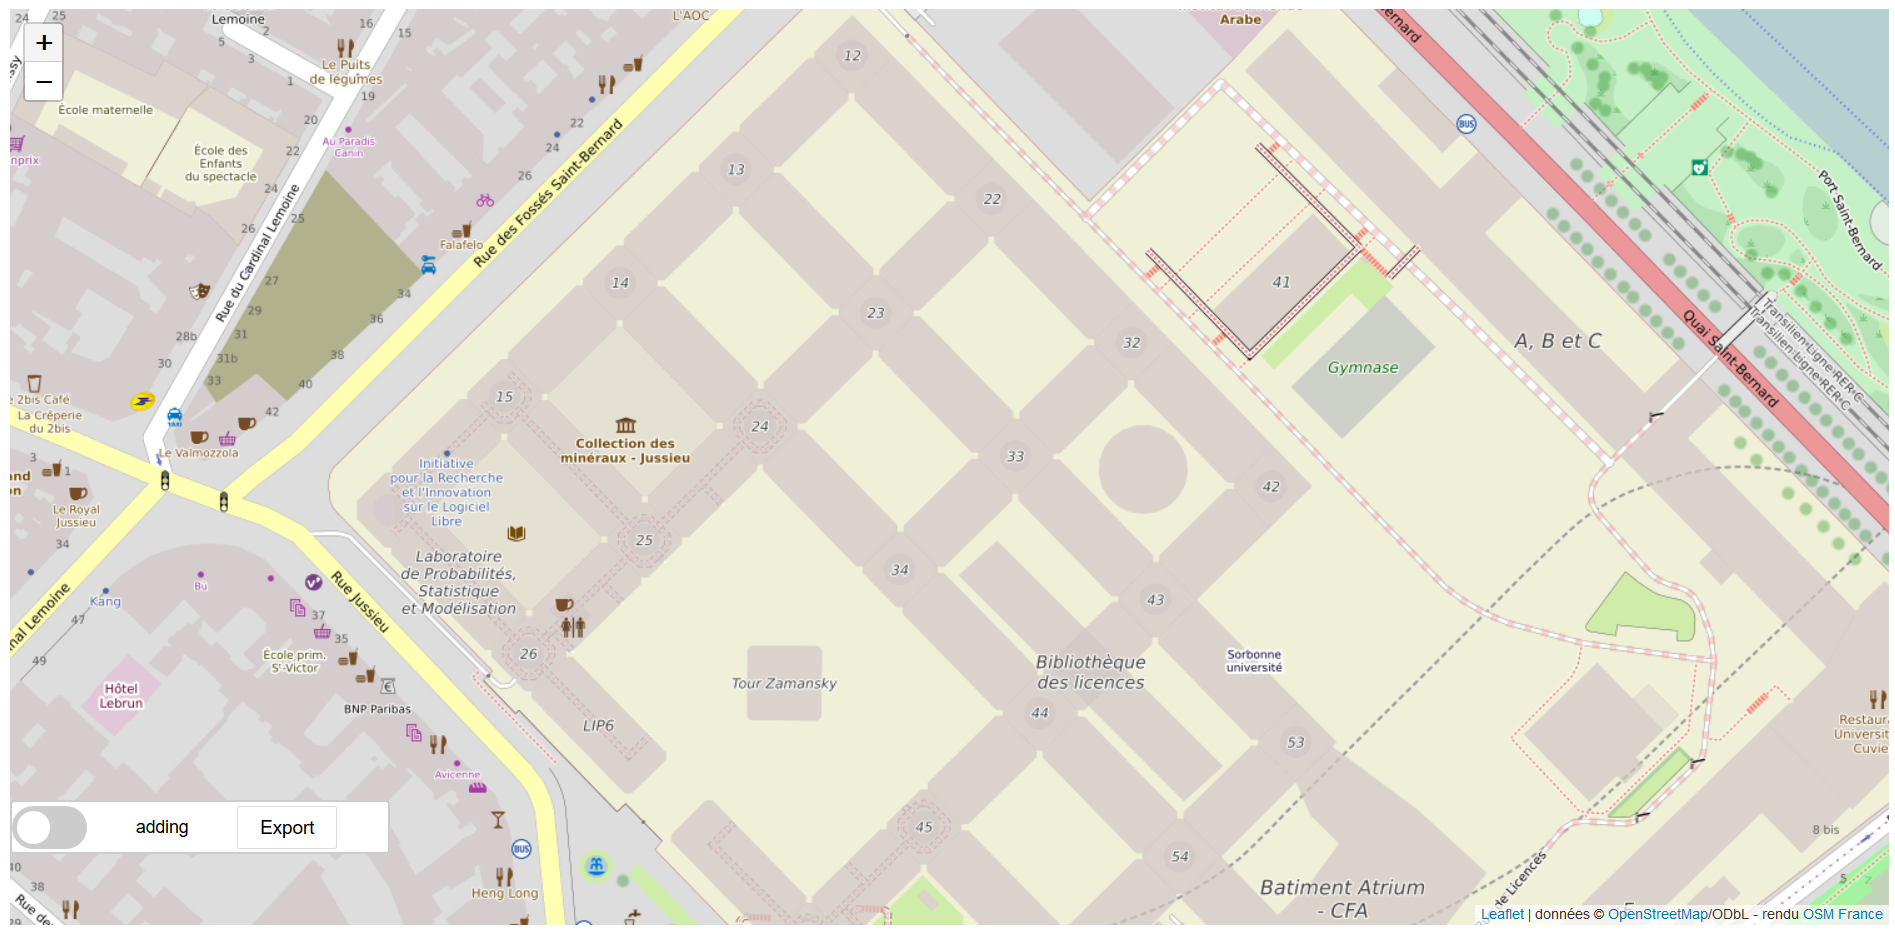
\includegraphics[scale=0.42]{capt1.PNG}
 	\caption{carte vierge}
 	\end{center}
	\end{figure}
	%________________
 	%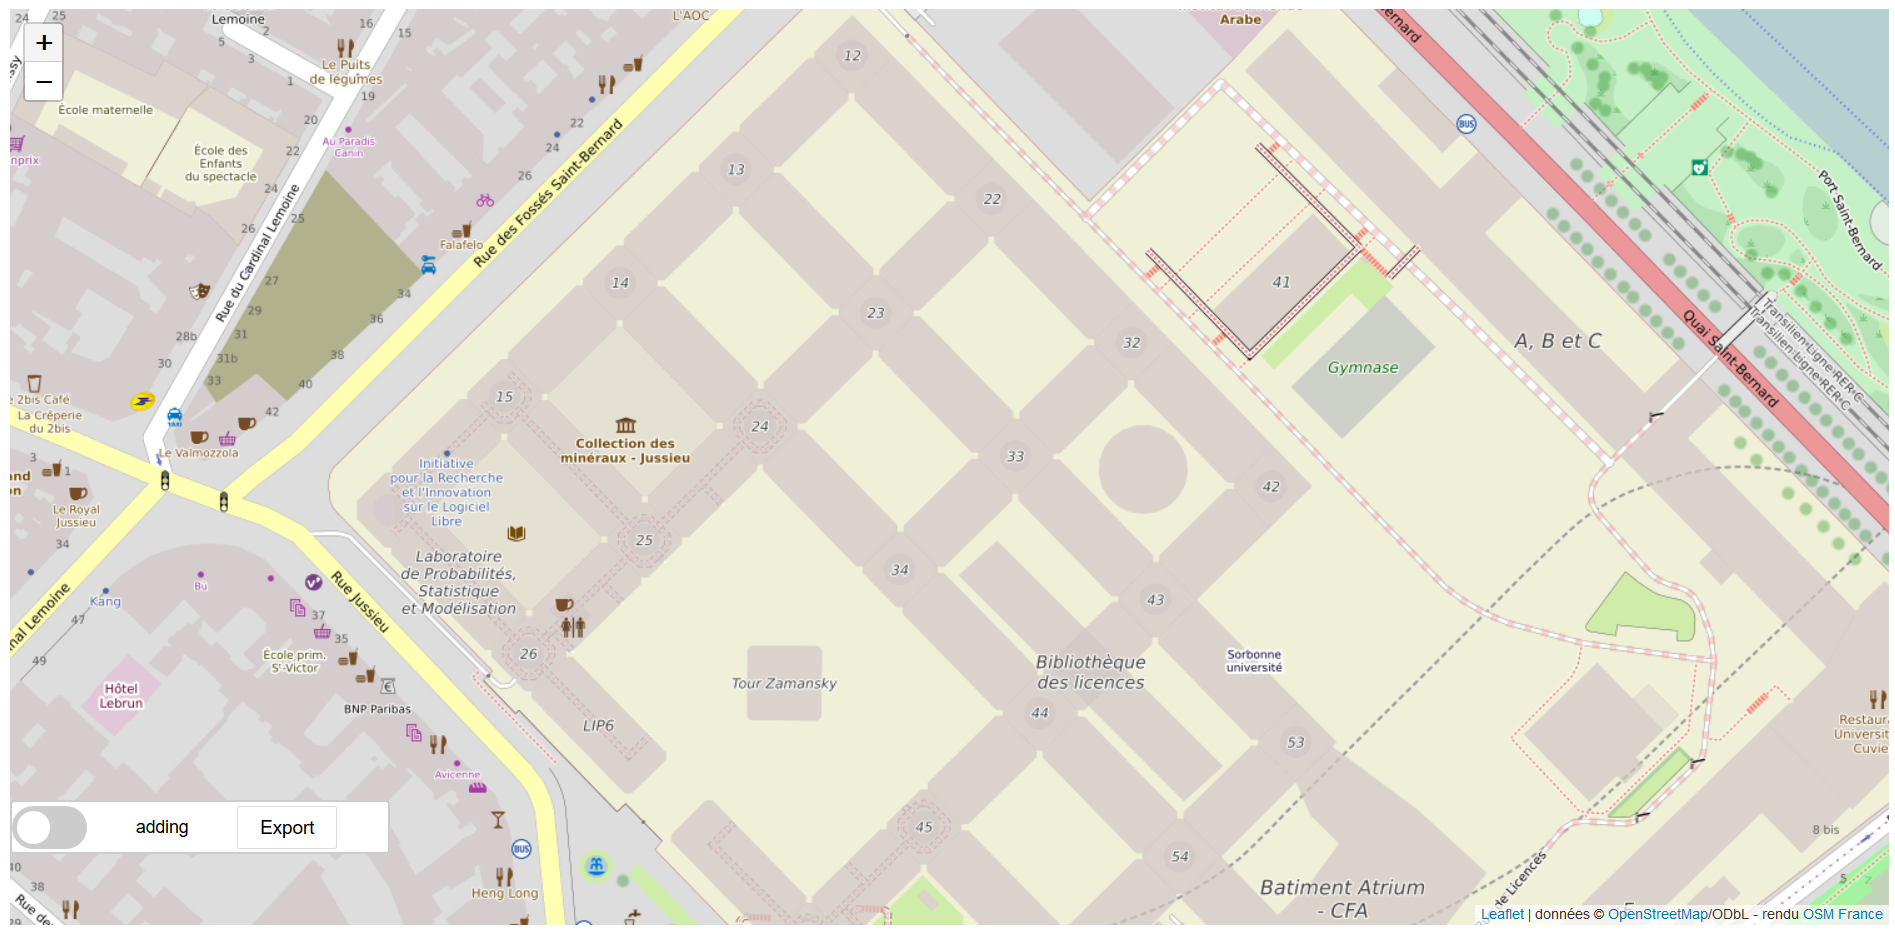
\includegraphics[scale=0.42]{capt1.PNG}\\
 	
 	La carte est interactive et on peut la déplacer avec la souris.
  Les boutons situés en haut à gauche permettent de zoomer et dézoomer sur la carte.\\ \\
 Le cadre situé en bas à gauche contient un switch (interrupteur) et un bouton : le switch permet de changer le mode d'interaction, et le bouton permet de finaliser le plan de vol en l'exportant dans un fichier.
 Il existe deux modes d'interraction :  le mode d'ajout et le mode de suppression. Le mode dans lequel on se situe est indiqué à coté du switch ("adding" / "removing").\\ \\
  En cliquant sur la carte, un marqueur est placé à l'endroit du clic. Chaque marqueur représente un point de passage du drone dans son itinéraire de vol. Les marqueurs peuvent être déplacés à la souris (drag and drop). Lors du survol de la souris sur un marqueur, une bulle indique son numéro d'ordre (0 pour le point de départ).\\
  	\begin{itemize}
 	\item En mode d'ajout, en cliquant sur un marqueur, on peut spécifier dans une boite de dialogue l'altitude à laquelle doit se situer le drone à ce point lors du vol.\\

 	\item En mode de suppression, en cliquant sur un marqueur, on supprime ce dernier. Les marqueurs sont alors automatiquement remis dans le bon ordre et le trajet est retracé.\\ \\ \\
	\end{itemize}
    \medbreak
   	%\newpage
   	%\vspace*{1cm}
   	\newpage
   	\item On place des marqueurs en cliquant aux endroits voulus sur la carte. Au survol d'un marqueur, la bulle comportant son numéro d'ordre apparait :
 	%________________
 	\begin{figure}[!h]
 	\begin{center}
 	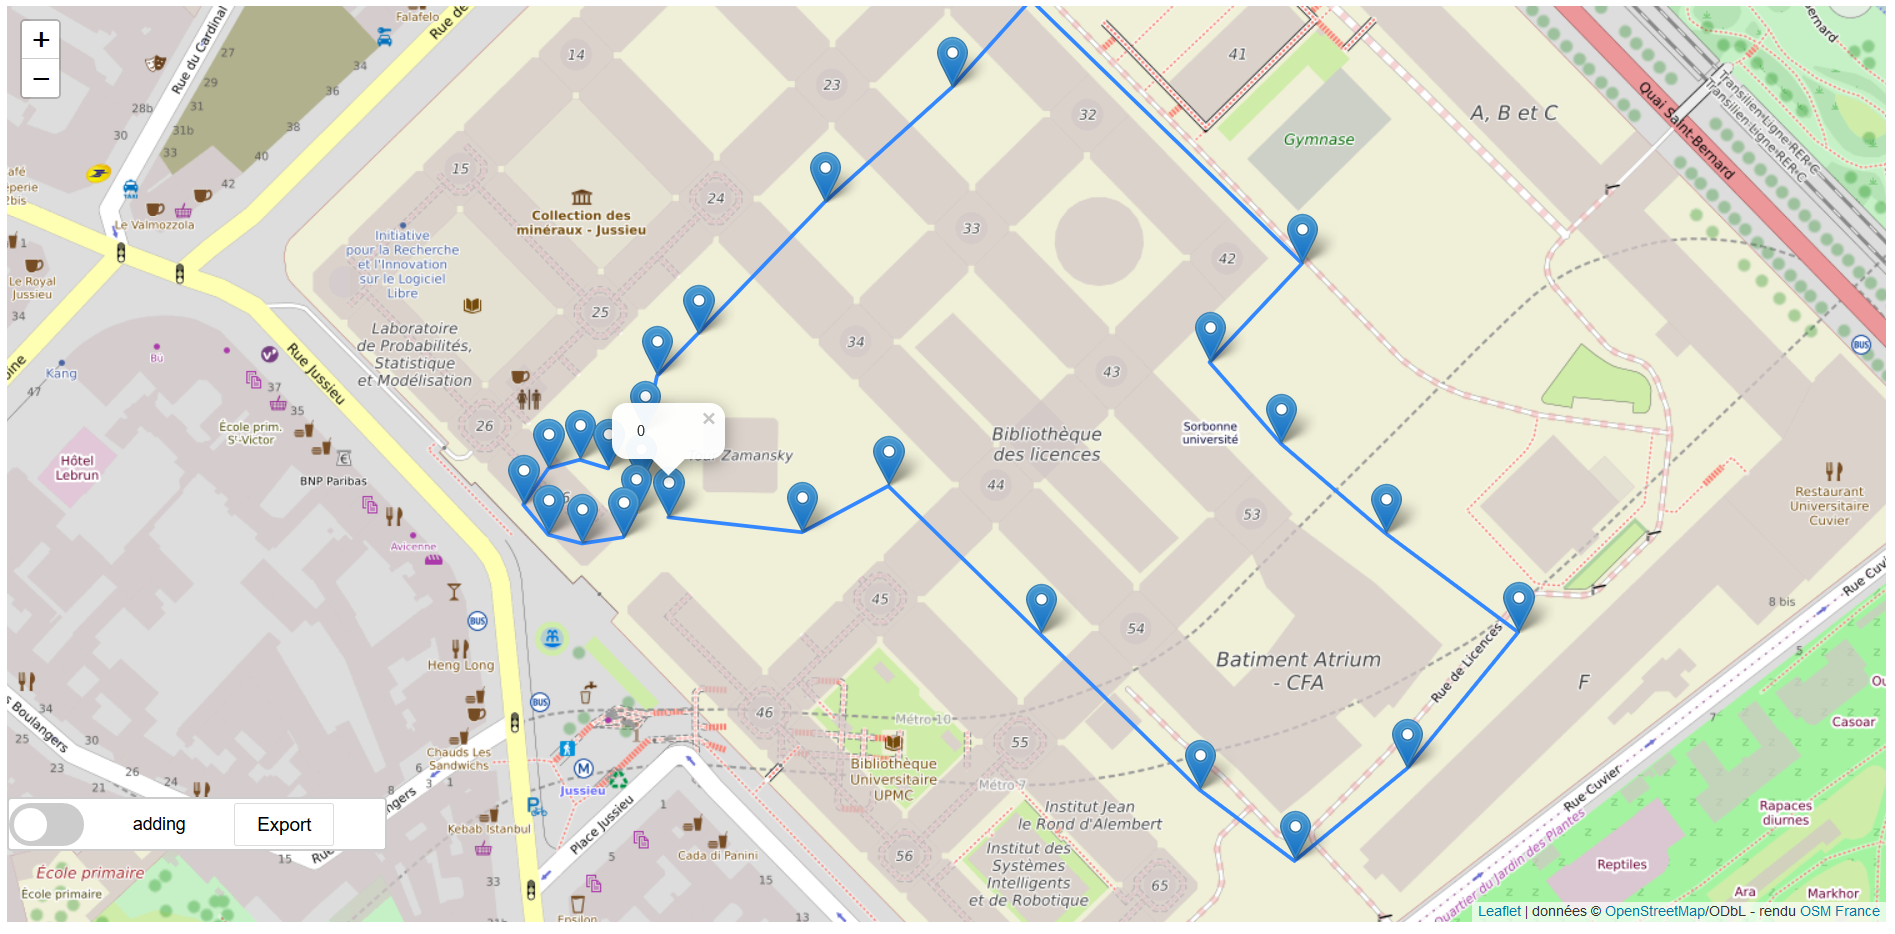
\includegraphics[scale=0.42]{capt3.PNG}
 	\caption{ajout de points de passage}
 	\end{center}
 	\end{figure}
 	%________________
 	%\vspace*{1.5cm}
 	
  	\item On souhaite retirer des marqueurs, on active le mode de suppression en cliquant sur le switch en bas à gauche (figure 4) et on clique ensuite sur les marqueurs à supprimer. L'ordre des marqueurs et le tracé du trajet s'adaptent :\\
	%________________	
	\begin{figure}[!h]
 	\begin{center}
 	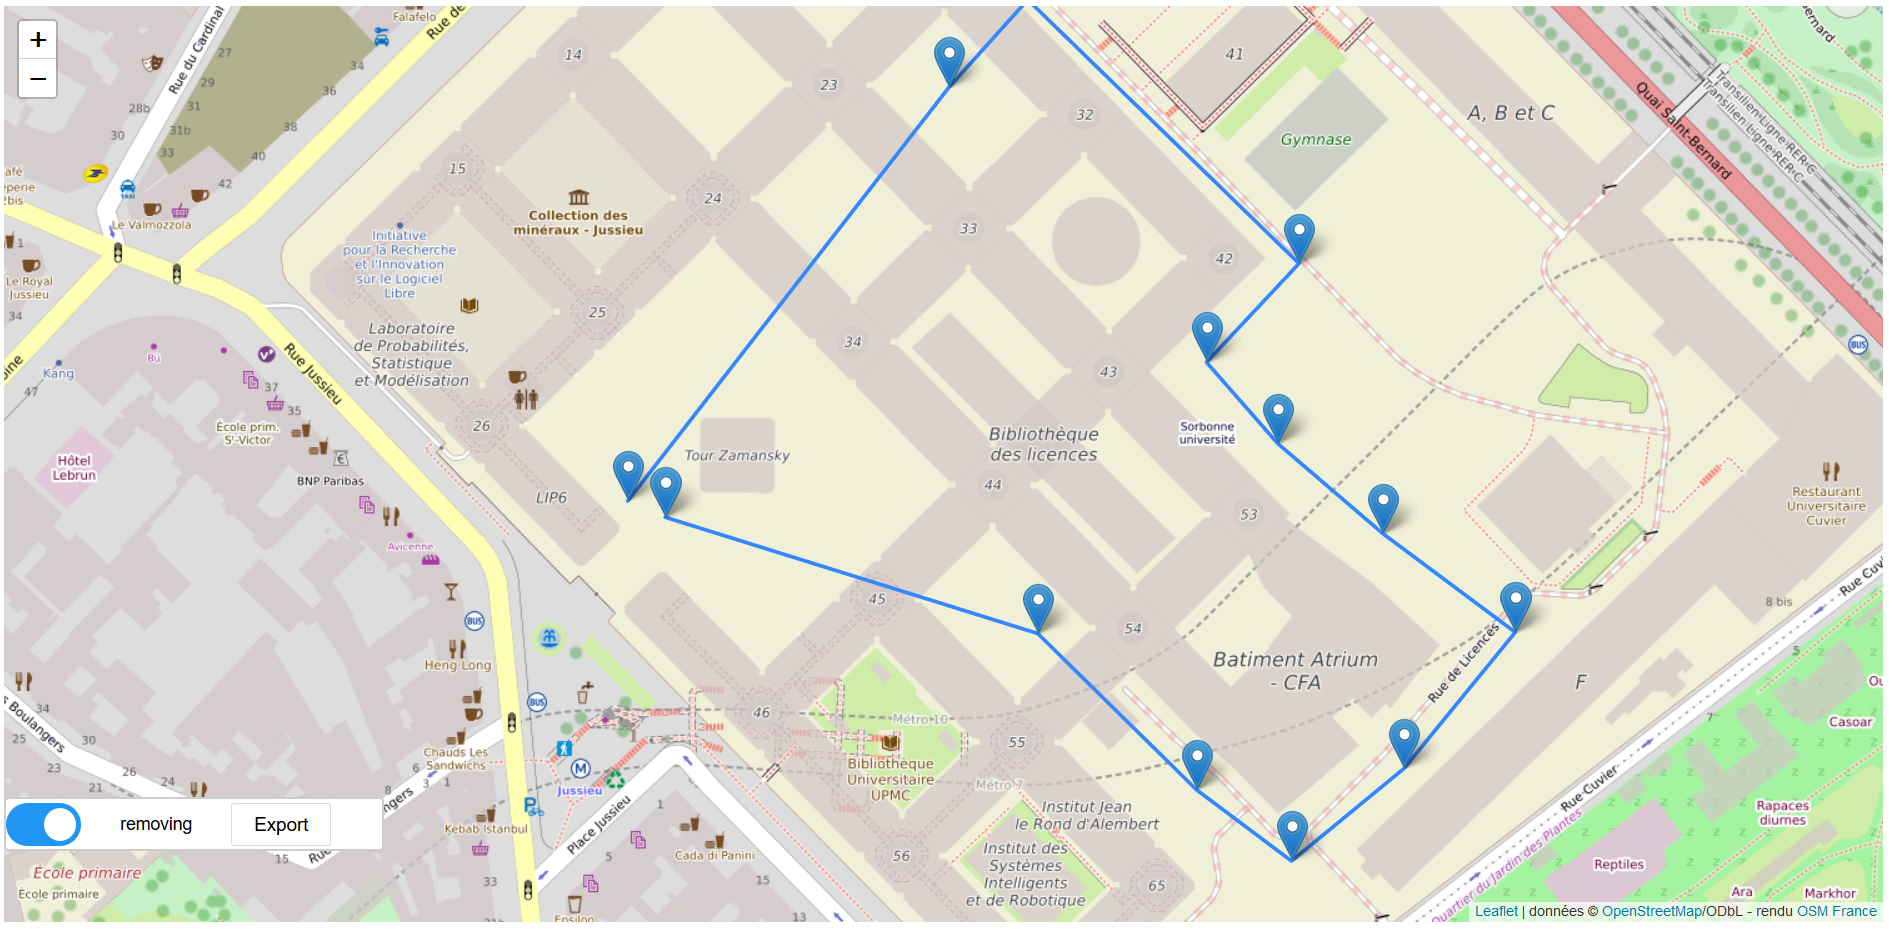
\includegraphics[scale=0.42]{capt5.PNG}
 	\caption{suppression de points de passage}
 	\end{center}
 	\end{figure}
 	%________________
	%\vspace*{0.5cm}
	\newpage
	\item On clique sur un marqueur pour spécifier l'altitude voulue à ce point (figure 5):
	%\vspace*{1cm}
	%________________
	\begin{figure}[!h]
 	\begin{center}
 	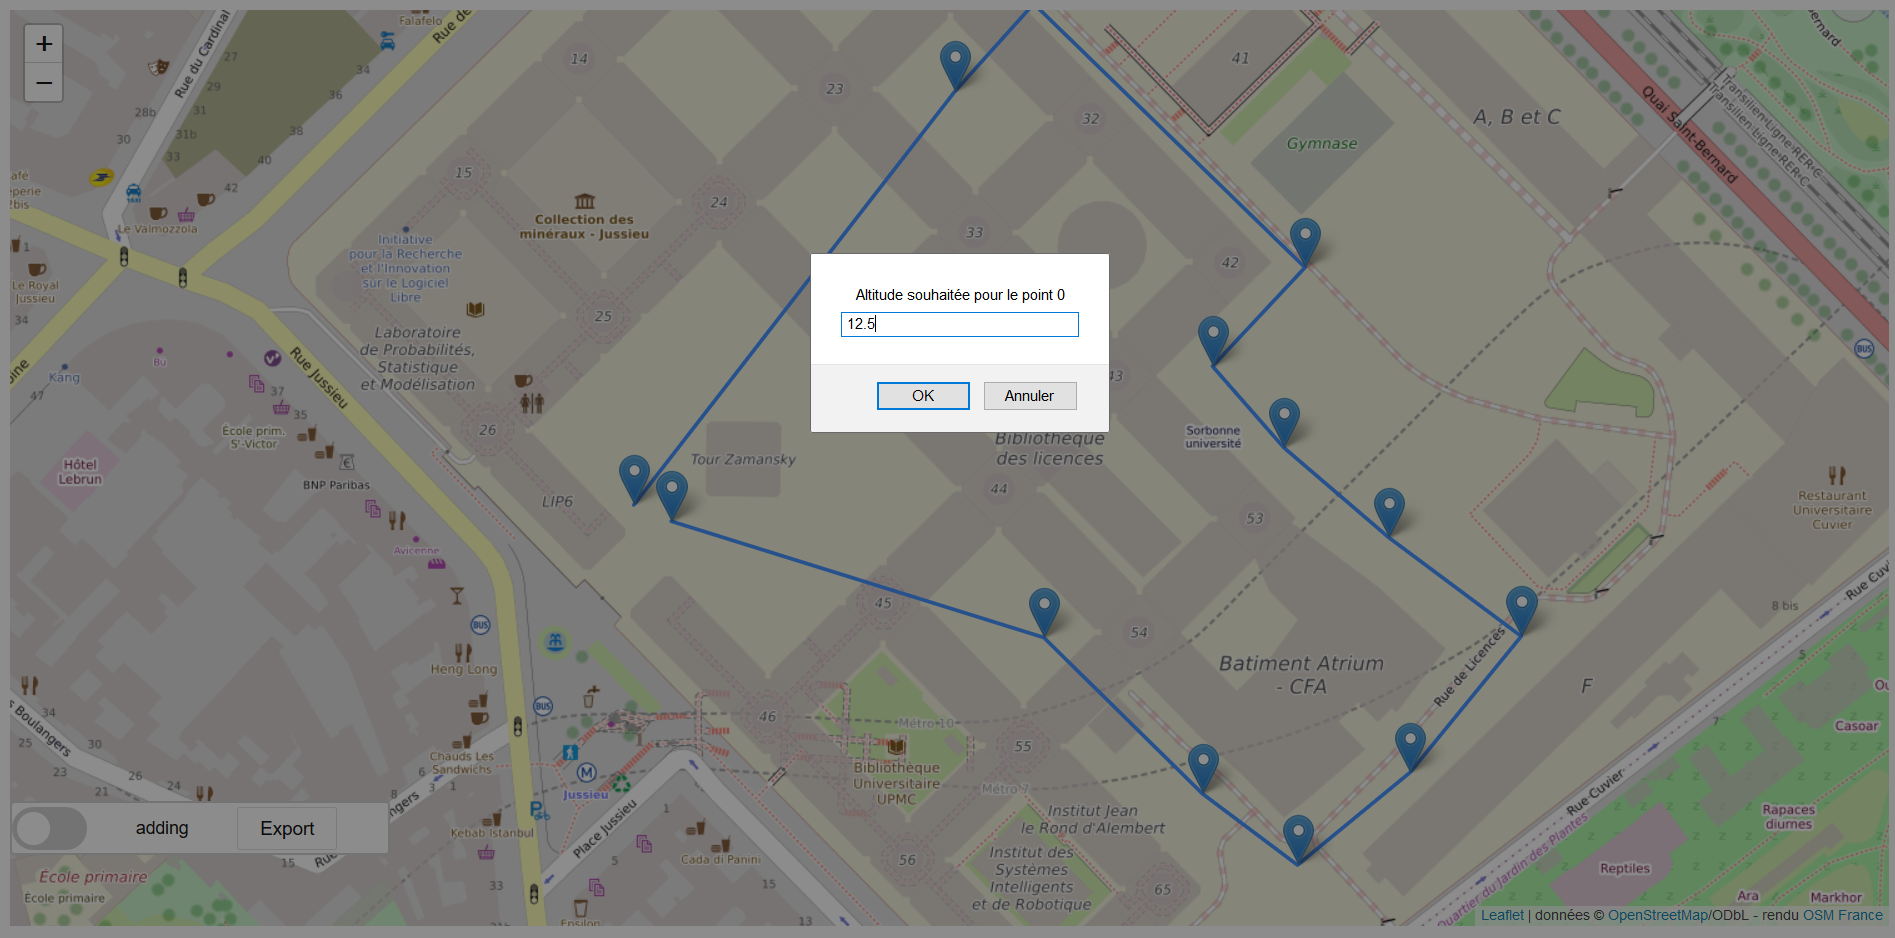
\includegraphics[scale=0.42]{capt6.PNG}
 	\caption{modification de l'altitude}
 	\end{center}
 	\end{figure}
 	%________________
 	
 	\item On peut déplacer les marqueurs avec un cliquer-glisser (drag and drop) sur ces derniers (figure 6):
 	%________________
 	\begin{figure}[!h]
 	\begin{center}
 	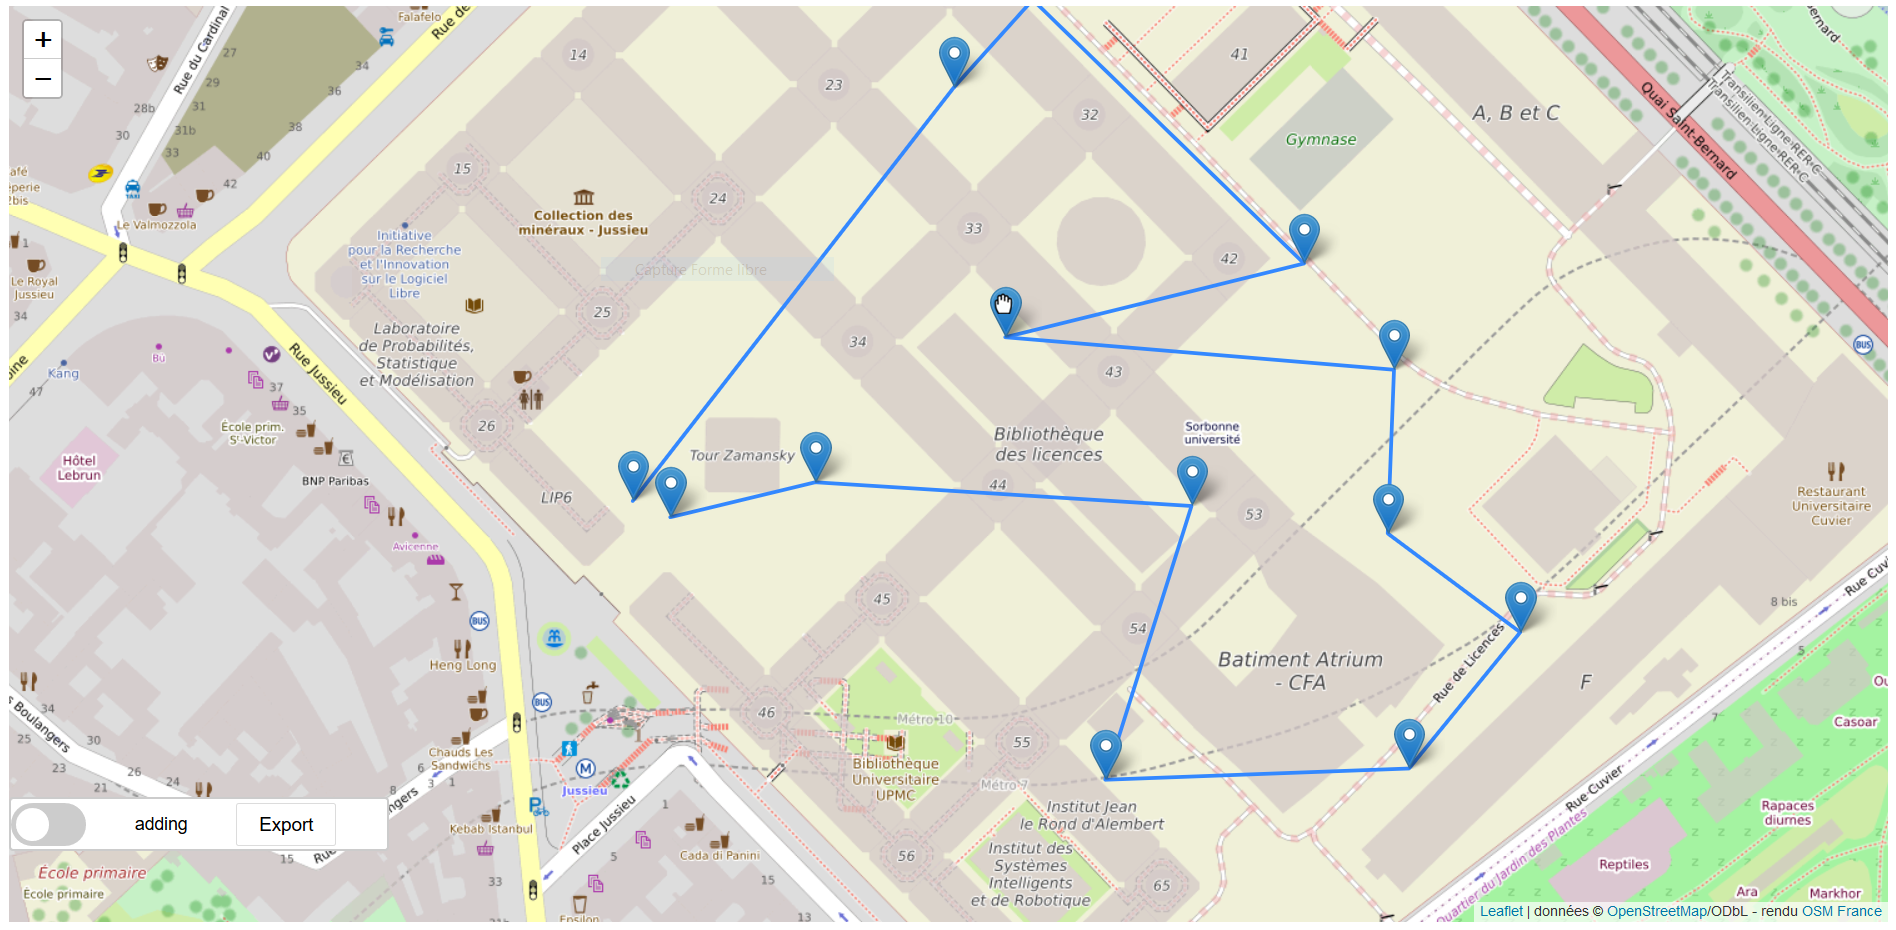
\includegraphics[scale=0.42]{capt7.PNG}
 	\caption{déplacer les marqueurs}
 	\end{center}
 	\end{figure}
 	%________________ 	
 	\newpage
  	%Une fois le plan de vol terminé, on clique sur le bouton pour obtenir le fichier correspondant au trajet défini :
  	\item Une fois le plan de vol terminé, on clique sur le bouton pour obtenir le fichier correspondant au trajet défini :
  	%________________
  	\begin{figure}[!h]
 	\begin{center}
 	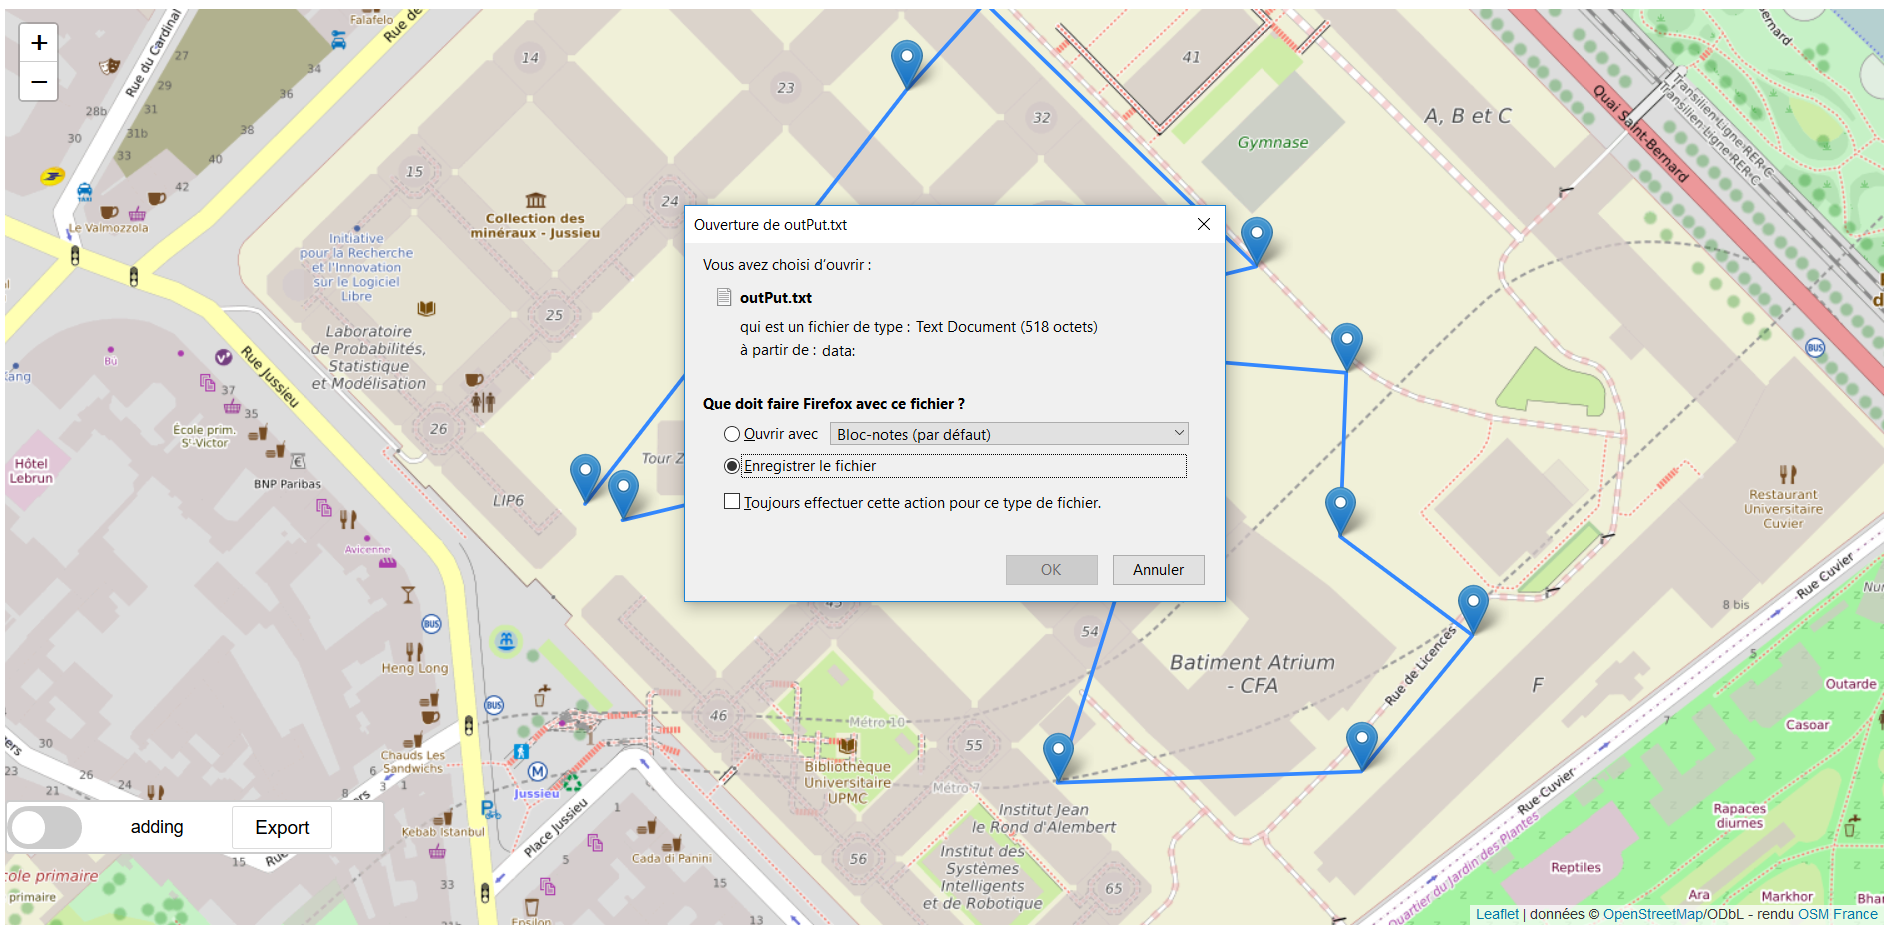
\includegraphics[scale=0.42]{capt8.PNG}
 	\caption{sauvegarde du plan}
 	\end{center}
 	\end{figure}
 	%________________ 	
 	\end{enumerate}
	\textit{Toutes ces images sont issues de prototypes d'interface graphique. Elles ne sont donc en aucun cas définitives et sont sujet à changement.}
\end{document}
